\documentclass[10pt,technote]{IEEEtran}
\usepackage{amssymb}
\usepackage{amsmath}
\usepackage[toc, page]{appendix}
\usepackage{graphicx}
\usepackage{subcaption}

\title{Coursework 2: Representation and Distance Metrics Learning }
\author{Timothee Gathmann \textit{(\textbf{tlg15}, 01061046)}\\ Luka Lagator\textit{ (\textbf{ll5915, }01108413)}}

\begin{document}

\maketitle
\begin{abstract}
In the aim of retrieving the most correct nearest neighbours of a labelled data point, different distance metrics were evaluated, without any training. The Mahalanobis distance was then implemented without and with training its distance matrix, and ultimately kernelised to possibly improve the nearest neighbour score. The distance metric optimisation didn't significantly improve on the euclidean metric, as it seemed that the data was already optimally represented.

\end{abstract}



\section{Problem formulation}
The features $X \in \mathbb{R}^{D X N}$ are readily available, and consist of a set of samples $x_i \in \mathbb{R}^D, i = 1, 2, ..., N$ corresponding to $N$ pictures of pedestrians. Each sample is assigned a ground-truth label $l(x_i) \in \mathbb{N}$ identifying the individual on the picture. The features are divided in a training subset $T$, a query subset $Q$ and a gallery subset $G$. Our goal is to minimise the retrieval error when performing retrieval experiments with the K-Nearest Neighbour algorithm \cite{Cover1967} at different ranks ($R = 1, 2, ..., 10 $), with different distance metrics. For a distance metric $d(x_i, x_j)$, the nearest neighbour $x_j \in X$ of $x_i$ is defined as
\begin{equation}
    \begin{aligned}
    n_0(x_i) = x_j \\
d(x_i, x_j) \le d(x_i, x_n), \forall x_n \in X - x_j
    \end{aligned}
\end{equation}
The $k$ nearest neighbours of $x_i \in X$ are :
\begin{equation}
    \begin{aligned}
    n_k(x_i) = \lbrace x_j, n_{k-1}\rbrace 
    \\
    d(x_i, x_j) \le d(x_i, x_n) \forall x_n \in X - n_k(x_i)
    \end{aligned}
\end{equation}
We define the mAp as
\begin{equation}
\begin{aligned}
    mAp & =   \frac{1}{N_Q}\sum^{N_Q}_{i, x_i \in Q}  \frac{1}{tot(x_i)}\sum^{N_G}_{j, x_j \in G}\rho(x_i, x_j)\frac{\sum^{j}_z\rho(x_i, x_z)}{j} \\ 
    tot(x_i)& = \sum^{N_G}_j\rho(x_i, x_j)
    \end{aligned}
\end{equation}
Where 
\begin{equation}
    \rho(x_i, x_z) =
    \begin{cases}
        1 & l(x_i) = l(x_z)\\
        0 & l(x_i) \neq l(x_z)
    \end{cases}
\end{equation}

It can be seen that, to minimise the mAp error, the feature space has to be transformed such that all points of same label lie the closest to each other, and all points of different labels lie the furthest from each other.
We can formulate our problem as a Distance Metric Learning problem. We define the set $S = \lbrace x_i, x_j, ...\rbrace, \rho(x_i, x_j) = 1$ and the set $D = \lbrace x_i, x_j, ...\rbrace,  \rho(x_i, x_j) = 0$
Then our problem is to solve:

\begin{equation}
\max \sum_{(x_i, x_j) \in D} d(x_i, x_j)
\end{equation}
And
\begin{equation}
\min \sum_{(x_i, x_j) \in S} d(x_i, x_j) < k, k \in \mathbb{R^+}
\end{equation}
The optimisable parameters depend on which function $d(x_i, x_j)$ is chosen, as well as which $k$ was chosen.

\section{Baseline experiments}

\subsection{Standard metrics}
The following metrics were considered as a baseline, without any transforms applied to the features:
\begin{enumerate}
    \item First order Minkowski
    \item Euclidean distance
    \item Cross Correlation similarity
    \item Cosine similarity
    \item Bilinear similarity
\end{enumerate}

We retrieved the k-nearest neighbours of the query features with the gallery features according to each baseline metric and calculated mAp for k = 1-15. The results can be seen in the figure \ref{fig:baseline_map}. Although all metrics perform in a similar trends as the rank of the nearest neighbour algorithm is changed, the Minkowsky metrics of order 1 and 2 perform better, surpassing constantly the third best performing cosine similarity by 10 percentage points. Bilinear Similarity metric was computed with the identity matrix and yielded the exact same results as cosine similarity, implying that normalisation by the 2-norm product makes no difference.
\begin{figure}
    \centering
    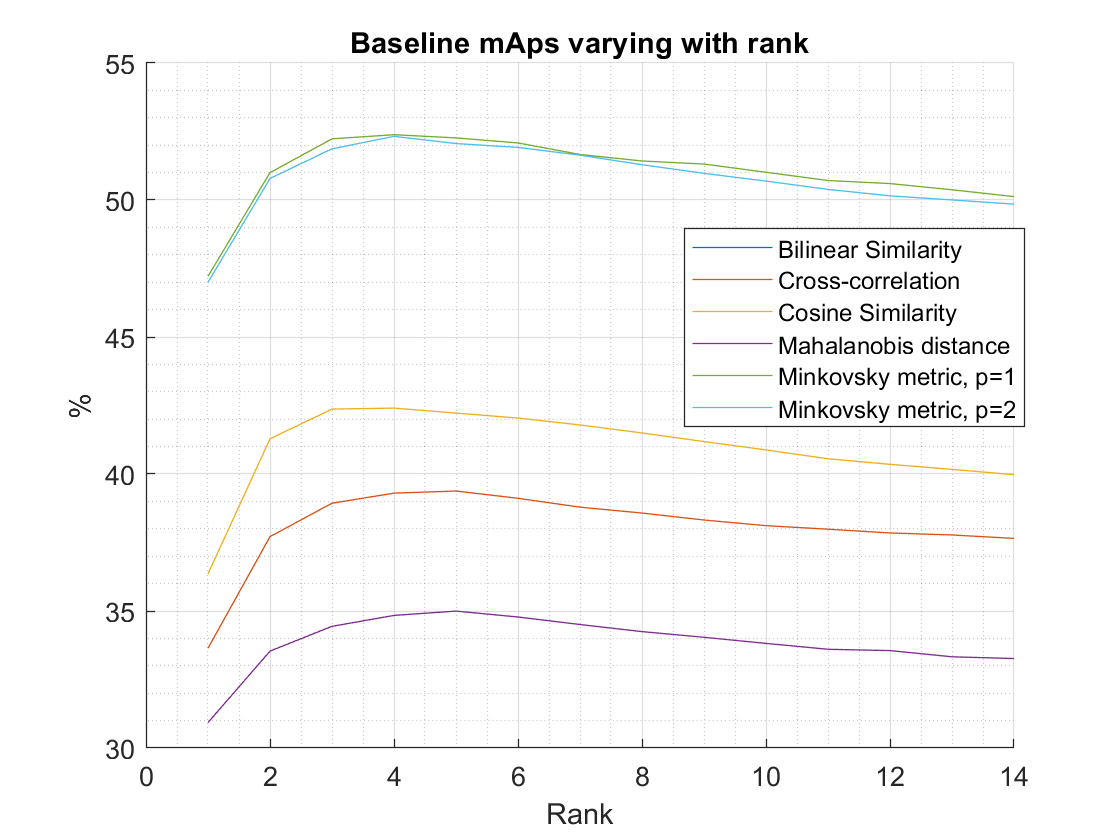
\includegraphics[width=\linewidth]{Graphs/mAp_vs_rank_baseline.png}
    \caption{Baseline mAps calculated at different ranks on testing data}
    \label{fig:baseline_map}
\end{figure}
\subsection{K-means}

\section{Improved approach: Kernel/Non-kernel Mahalanobis distance}
Mahalanobis distance learning was chosen as an attempt to improve the baseline metric, by learning the feature transformation that would improve the Euclidian distance metric. This seemed sensible as Euclidian distance was already 
Where this distance is defined by:
\begin{equation}
    d_A(x, y) = (x - y)^TA(x - y)
\end{equation}
and $A \in \mathbb{R}^{DXD}$, $A \ge 0$
\subsection{Without iterative training: choosing the right A matrix}
It was first explored what performance could be achieved by simply choosing a good A matrix and not not train it any further. Two options were compared:
\begin{enumerate}
    \item $A = I \rightarrow d_A(x, y) = ||x - y||_2^2$
    \item $A = cov(x \in T)^{-1}$
\end{enumerate}
Their respective performance on the test dataset are displayed in figure \ref{fig:maha_map}. 

\begin{figure}
    \centering
    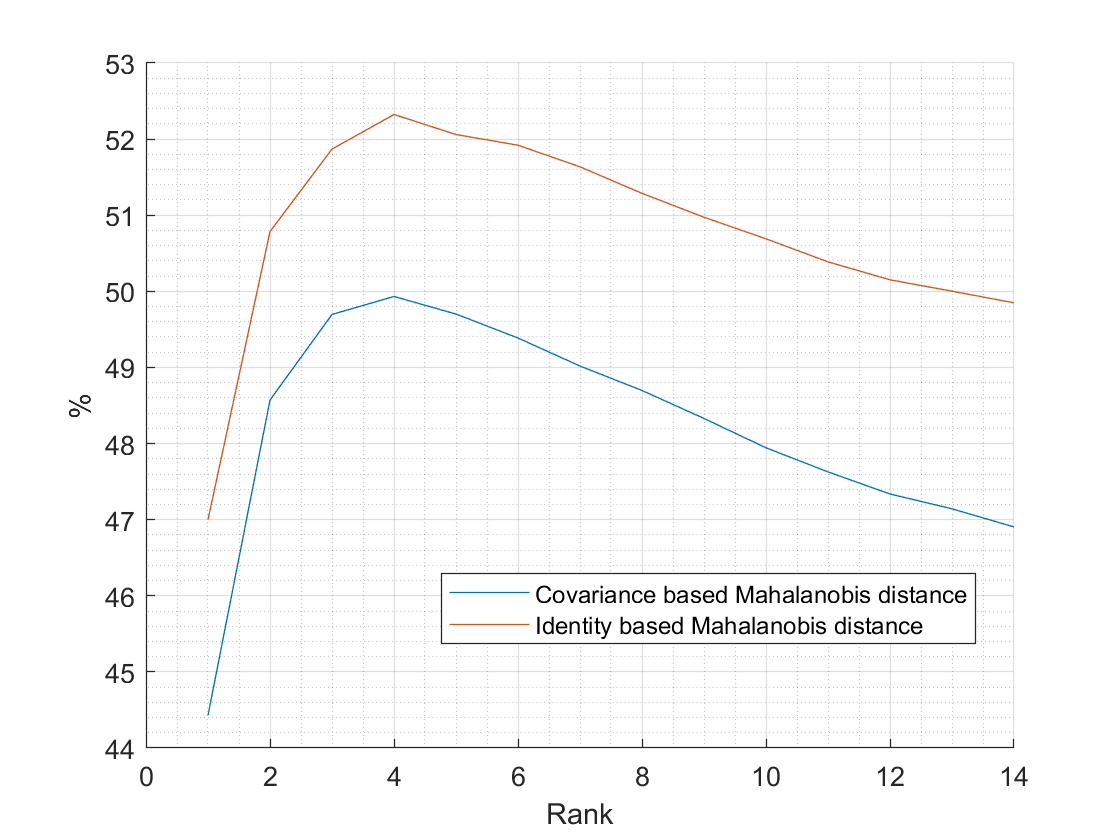
\includegraphics[width=\linewidth]{Graphs/maha_Map.png}
    \caption{mAps calculated at different ranks on the testing data. The metric being tested is the Mahalanobis distance with two different A matrices}
    \label{fig:maha_map}
\end{figure}

In the case $A = I$, the Malahanobis metric is the Euclidian distance as shown in figure \ref{fig:baseline_map}. In comparison, the covariance based Mahalanobis metric doesn't show promising result. One reason for that might be that the features are already strongly decorrelated, and the covariance matrix does not apply any linear transformation to the features other than scaling each feature by the inverse of its variance (only diagonal elements in the covariance matrix). 

Following this we attempted to learn the matrix A through constrained optimisation. The objective function to minimise was the following:

\begin{equation}
    \min_{A}\sum_{(x_i, x_j) \in S}{d_A (x_i, x_j)}
\end{equation}
s.t.
\begin{equation}
    \begin{aligned}
        d_A{(x_i, x_k)} - d_A (x_i, x_j) \ge 1 \forall(x_i, x_j, x_k) \in{\mathbb{R}}  \\
        A \ge 0 \\
        where (x_i, x_j) \in S, (x_i, x_k) \in D
    \end{aligned}
\end{equation}
The optimisation problem was implemented as: 
\begin{equation}
    \begin{aligned}
    \min_{J,\lambda} L \\
    L(A, \lambda)  = \sum_{d_A \in D_s}d_A - |\lambda|C \\
        C = \sum_{}d_A{(x_i, x_k)} - d_A (x_i, x_j) -1,  \forall(x_j, x_k)  \\ \text{at 100 randomly chosen i}
    \end{aligned}
\end{equation}

The first term is the sum of distances between similar points (denoted by set Ds). The second term forms the sum of randomly generated constraints parameterised by $\lambda$, as all the constraint calculations could not be held in memory during runtime. The parameters for optimisation are the elements of A, used for distance computation, and the parameter $\lambda$. The optimisation was tested on three cases; with no kernel, as well as with the Gaussian and Polynomial kernels. With kernel learning, the variance $\sigma$ and power $p$ were scalar parameters to be optimised as well. The matrix A was initialised as either training data covariance matrix or as an identity matrix. The parameters l was initialised to 1, and kernel parameters $\sigma$ and $p$ to 30 and 0.1 respectively, when needed. $\sigma$ was chosen by inspection to prevent extreme values ([0,1]) as starting values for the kernel. Similarly $p$ was chosen to prevent tendency to $\inf$ of kernel function values.
Figure \ref{fig:comparison_init} shows the results of the three cases for two different initialisations of matrix A. We can see that the polynomial kernel does not perform well. In comparison, using no kernel or gaussian kernel yields better results, where  the gaussian kernel tends to do a bit better.
All the mAp for the testing data was calculated by kNN retrieval for $k = 10$.
The best result was achieved by the gaussian kernel learning when the A matrix was initialised as I.

\begin{figure}
\begin{subfigure}{\linewidth}
    \centering
    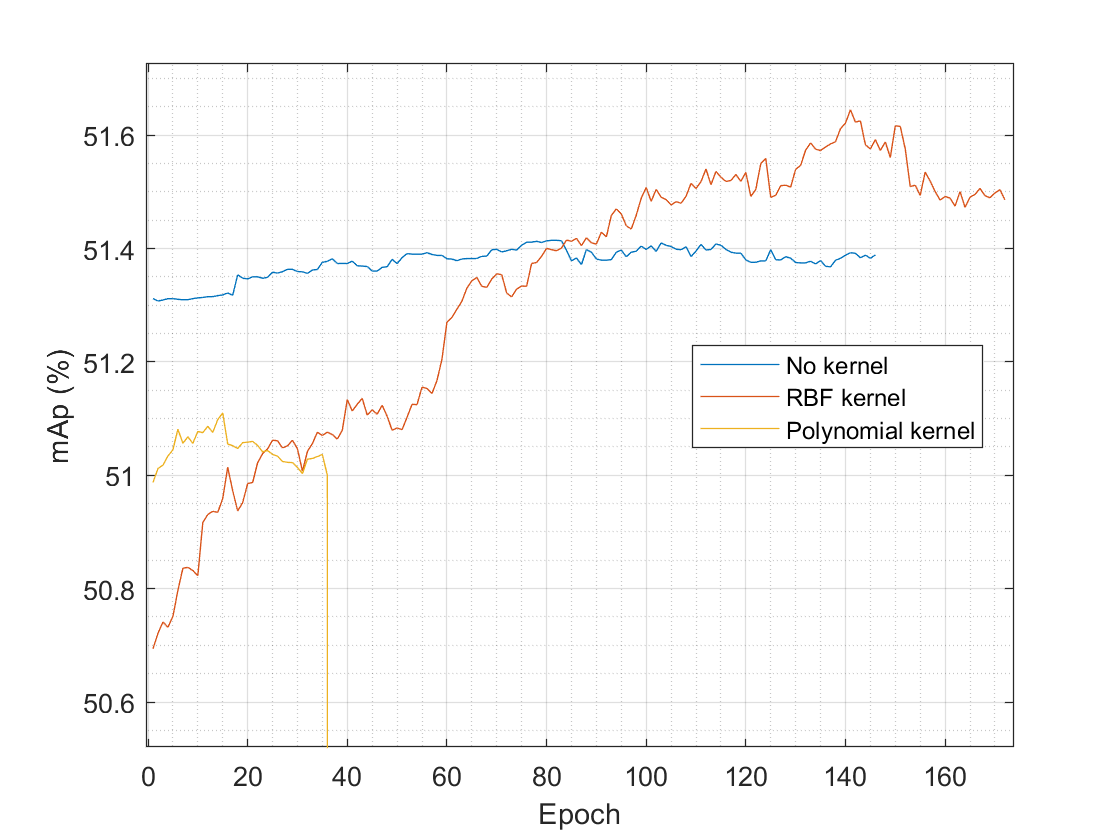
\includegraphics[width=\linewidth]{Graphs/I_init_comparison.png}
    
    
\end{subfigure}
\begin{subfigure}{\linewidth}
    \centering
    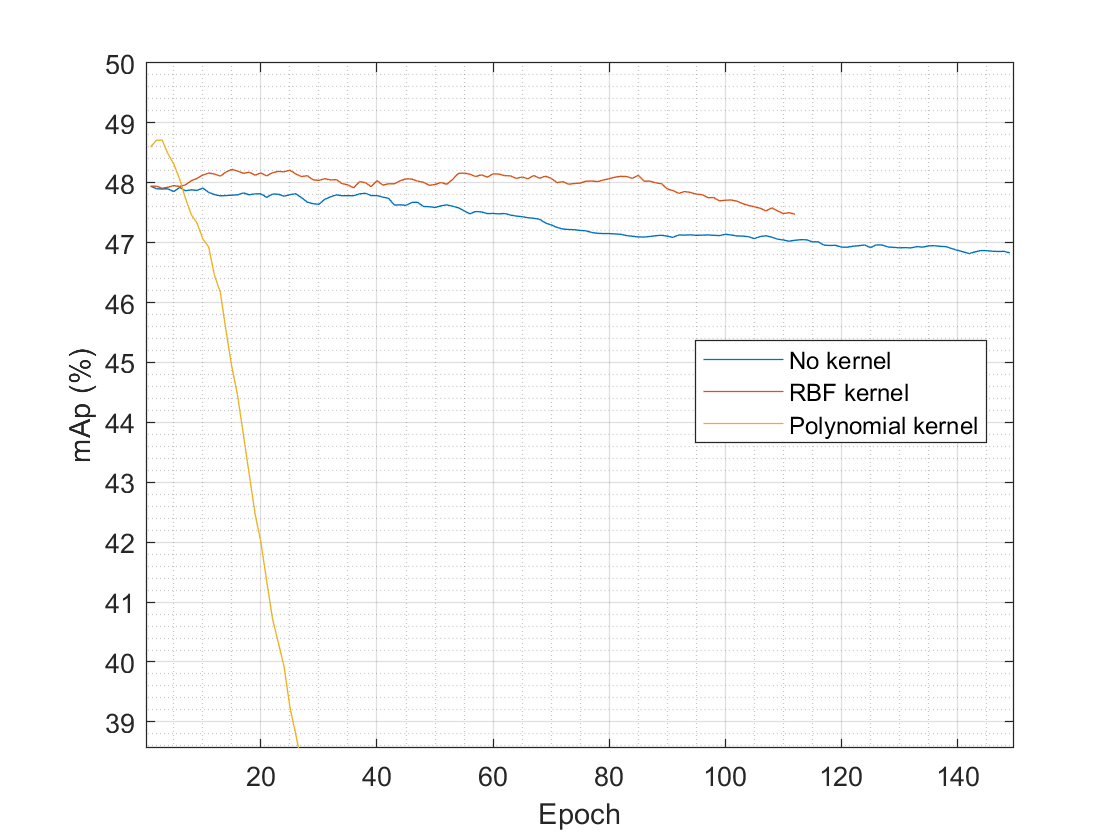
\includegraphics[width=\linewidth]{Graphs/cov_init_comparison.png}
\end{subfigure}
\caption{Evolution of mAp with the number of optimisation iterations, for the Mahalanobis distance initialised with the identity matrix (top) and the covariance matrix (bottom). The variants with no kernel, RBF kernel and polynomial kernel are shown.}
\label{fig:comparison_init}
\end{figure}
\begin{table}
    \centering
    \begin{tabular}{c|c}
        Euclidean distance & RBF Kernel Mahalanobis distance \\
        50.64\% & 51.64 \%
    \end{tabular}
    \caption{Comparison of the mAp of the euclidean distance and our improved RBF kernel Mahalanobis distance initialised with an identity matrix}
    \label{tab:my_label}
\end{table}
\appendices

\section{Optimisation of computations}

The deep learning platform PyTorch was used to perform most the large-scale matrix algebra as well as the optimisation. This platform allowed higher computation speeds by enabling computation graphs and making use of the parallel computing capabilities of our GPU.
The initial experiment was done by attempting to minimise the following objective function: \begin{equation}
    loss = l*\sum_{d \in S}d -  \sum_{d \in D}\sqrt{d}
\end{equation}
where set S contains all computed distances between similar data points and set D contains all the distances between dissimilar data points. This was a rudimentary implementation of the constrained optimisation problem defined as
\begin{equation}
    \max_{A}\sum_{(x_i, x_j) \in D}\sqrt{d_A (x_i, x_j)}
\end{equation}
s.t.
\begin{equation}
    \begin{aligned}
        c(A) = \sum_{(x_i, x_j) \in S}d_A (x_i, x_j) \le 1 \\
        A \ge 0
    \end{aligned}
\end{equation}
The A matrix was initialised as the 
inverse covariance matrix of the training features and decomposed by Cholesky decomposition to obtain the upper triangular matrix L. After transforming the training data points by L, Euclidian distance is computed on the transformed data points as follows:
\begin{equation}
    |Lx_i - Lx_j|_2^2 = \sum_{i}(Lx_i)^2 + \sum_{j}(Lx_j)^2 - 2(Lx_i)^T(Lx_j)
\end{equation}
The expansion on the right hand side ignores the square root operation in 2-norm computation. The square terms are first computed for all the training data points contained in the data matrix X and the last term is found as the matrix product of $X^TX$. This result gives the distance matrix of size $NxN$ where N is the number of training points. The diagonal is set to 0, as it should be when $x_i = x_j$, to stabilise the optimisation, since (due to computational precision) the summation of the first two terms slightly differs to the summation in the matrix product. 


\bibliographystyle{IEEEtran}
\bibliography{refs}
\end{document}
